\documentclass[12pt]{article}
\usepackage[margin=0.1in]{geometry}
\usepackage{xcolor}
\usepackage{framed}
\usepackage{enumitem}
\usepackage{adjustbox}
\usepackage{natbib}
\usepackage{chngpage}
\usepackage{mathtools,xparse}
\usepackage{graphics}
\usepackage{tikz}
\usepackage{tikz-cd}
\colorlet{shadecolor}{orange!15}
% \definecolor{shadecolor}{rgb}{255,128,0}\
\usepackage{float}
\usepackage{fullpage} % Package to use full page
\usepackage{parskip} % Package to tweak paragraph skipping
\usepackage{amsmath}
\usepackage{amssymb}
\usepackage{hyperref}
\usepackage{pdflscape}
\usepackage{setspace}
\usepackage{graphicx} % Allows including images
\usepackage{booktabs} % Allows the use of \toprule, \midrule and \bottomrule in tables
\usepackage{longtable}
\usepackage{indentfirst}
\usetikzlibrary{arrows,shapes,positioning,shadows,trees}
\usepackage{array}
\newcommand{\PreserveBackslash}[1]{\let\temp=\\#1\let\\=\temp}
\newcolumntype{L}[1]{>{\PreserveBackslash\raggedright}m{#1}}
\newcolumntype{R}[1]{>{\PreserveBackslash}p{#1}}
\newcolumntype{C}[1]{>{\PreserveBackslash\centering}m{#1}}

\newcommand{\mc}[3]{\multicolumn{#1}{#2}{#3}}

\tikzset{
  basic/.style  = {draw, text width=2cm, drop shadow, font=\sffamily, rectangle},
  root/.style   = {basic, rounded corners=2pt, thin, align=center,
                   fill=green!30},
  level 2/.style = {basic, rounded corners=6pt, thin,align=center, fill=green!60,
                   text width=8em},
  level 3/.style = {basic, thin, align=left, fill=pink!60, text width=6.5em}
}


\newcommand\independent{\protect\mathpalette{\protect\independenT}{\perp}}
\newcommand\gamij{\mathbf{\gamma_{ij}}}
\def\independenT#1#2{\mathrel{\rlap{$#1#2$}\mkern2mu{#1#2}}}
\newcommand\params{(p_M, p_{M\ell}, p_{U\ell})}
\newcommand\longparam{(L,n_1,n_2, p_M,p_{M\ell},p_{U\ell})}


%Allows multi-column tables 
% Macros for Scientific Word and Scientific WorkPlace 5.5 documents saved with the LaTeX filter.
% Copyright (C) 2005 Mackichan Software, Inc.

\typeout{TCILATEX Macros for Scientific Word and Scientific WorkPlace 5.5 <06 Oct 2005>.}
\typeout{NOTICE:  This macro file is NOT proprietary and may be 
freely copied and distributed.}
%
\makeatletter

%%%%%%%%%%%%%%%%%%%%%
% pdfTeX related.
\ifx\pdfoutput\relax\let\pdfoutput=\undefined\fi
\newcount\msipdfoutput
\ifx\pdfoutput\undefined
\else
 \ifcase\pdfoutput
 \else 
    \msipdfoutput=1
    \ifx\paperwidth\undefined
    \else
      \ifdim\paperheight=0pt\relax
      \else
        \pdfpageheight\paperheight
      \fi
      \ifdim\paperwidth=0pt\relax
      \else
        \pdfpagewidth\paperwidth
      \fi
    \fi
  \fi  
\fi

%%%%%%%%%%%%%%%%%%%%%
% FMTeXButton
% This is used for putting TeXButtons in the 
% frontmatter of a document. Add a line like
% \QTagDef{FMTeXButton}{101}{} to the filter 
% section of the cst being used. Also add a
% new section containing:
%     [f_101]
%     ALIAS=FMTexButton
%     TAG_TYPE=FIELD
%     TAG_LEADIN=TeX Button:
%
% It also works to put \defs in the preamble after 
% the \input tcilatex
\def\FMTeXButton#1{#1}
%
%%%%%%%%%%%%%%%%%%%%%%
% macros for time
\newcount\@hour\newcount\@minute\chardef\@x10\chardef\@xv60
\def\tcitime{
\def\@time{%
  \@minute\time\@hour\@minute\divide\@hour\@xv
  \ifnum\@hour<\@x 0\fi\the\@hour:%
  \multiply\@hour\@xv\advance\@minute-\@hour
  \ifnum\@minute<\@x 0\fi\the\@minute
  }}%

%%%%%%%%%%%%%%%%%%%%%%
% macro for hyperref and msihyperref
%\@ifundefined{hyperref}{\def\hyperref#1#2#3#4{#2\ref{#4}#3}}{}

\def\x@hyperref#1#2#3{%
   % Turn off various catcodes before reading parameter 4
   \catcode`\~ = 12
   \catcode`\$ = 12
   \catcode`\_ = 12
   \catcode`\# = 12
   \catcode`\& = 12
   \catcode`\% = 12
   \y@hyperref{#1}{#2}{#3}%
}

\def\y@hyperref#1#2#3#4{%
   #2\ref{#4}#3
   \catcode`\~ = 13
   \catcode`\$ = 3
   \catcode`\_ = 8
   \catcode`\# = 6
   \catcode`\& = 4
   \catcode`\% = 14
}

\@ifundefined{hyperref}{\let\hyperref\x@hyperref}{}
\@ifundefined{msihyperref}{\let\msihyperref\x@hyperref}{}




% macro for external program call
\@ifundefined{qExtProgCall}{\def\qExtProgCall#1#2#3#4#5#6{\relax}}{}
%%%%%%%%%%%%%%%%%%%%%%
%
% macros for graphics
%
\def\FILENAME#1{#1}%
%
\def\QCTOpt[#1]#2{%
  \def\QCTOptB{#1}
  \def\QCTOptA{#2}
}
\def\QCTNOpt#1{%
  \def\QCTOptA{#1}
  \let\QCTOptB\empty
}
\def\Qct{%
  \@ifnextchar[{%
    \QCTOpt}{\QCTNOpt}
}
\def\QCBOpt[#1]#2{%
  \def\QCBOptB{#1}%
  \def\QCBOptA{#2}%
}
\def\QCBNOpt#1{%
  \def\QCBOptA{#1}%
  \let\QCBOptB\empty
}
\def\Qcb{%
  \@ifnextchar[{%
    \QCBOpt}{\QCBNOpt}%
}
\def\PrepCapArgs{%
  \ifx\QCBOptA\empty
    \ifx\QCTOptA\empty
      {}%
    \else
      \ifx\QCTOptB\empty
        {\QCTOptA}%
      \else
        [\QCTOptB]{\QCTOptA}%
      \fi
    \fi
  \else
    \ifx\QCBOptA\empty
      {}%
    \else
      \ifx\QCBOptB\empty
        {\QCBOptA}%
      \else
        [\QCBOptB]{\QCBOptA}%
      \fi
    \fi
  \fi
}
\newcount\GRAPHICSTYPE
%\GRAPHICSTYPE 0 is for TurboTeX
%\GRAPHICSTYPE 1 is for DVIWindo (PostScript)
%%%(removed)%\GRAPHICSTYPE 2 is for psfig (PostScript)
\GRAPHICSTYPE=\z@
\def\GRAPHICSPS#1{%
 \ifcase\GRAPHICSTYPE%\GRAPHICSTYPE=0
   \special{ps: #1}%
 \or%\GRAPHICSTYPE=1
   \special{language "PS", include "#1"}%
%%%\or%\GRAPHICSTYPE=2
%%%  #1%
 \fi
}%
%
\def\GRAPHICSHP#1{\special{include #1}}%
%
% \graffile{ body }                                  %#1
%          { contentswidth (scalar)  }               %#2
%          { contentsheight (scalar) }               %#3
%          { vertical shift when in-line (scalar) }  %#4

\def\graffile#1#2#3#4{%
%%% \ifnum\GRAPHICSTYPE=\tw@
%%%  %Following if using psfig
%%%  \@ifundefined{psfig}{\input psfig.tex}{}%
%%%  \psfig{file=#1, height=#3, width=#2}%
%%% \else
  %Following for all others
  % JCS - added BOXTHEFRAME, see below
    \bgroup
	   \@inlabelfalse
       \leavevmode
       \@ifundefined{bbl@deactivate}{\def~{\string~}}{\activesoff}%
        \raise -#4 \BOXTHEFRAME{%
           \hbox to #2{\raise #3\hbox to #2{\null #1\hfil}}}%
    \egroup
}%
%
% A box for drafts
\def\draftbox#1#2#3#4{%
 \leavevmode\raise -#4 \hbox{%
  \frame{\rlap{\protect\tiny #1}\hbox to #2%
   {\vrule height#3 width\z@ depth\z@\hfil}%
  }%
 }%
}%
%
\newcount\@msidraft
\@msidraft=\z@
\let\nographics=\@msidraft
\newif\ifwasdraft
\wasdraftfalse

%  \GRAPHIC{ body }                                  %#1
%          { draft name }                            %#2
%          { contentswidth (scalar)  }               %#3
%          { contentsheight (scalar) }               %#4
%          { vertical shift when in-line (scalar) }  %#5
\def\GRAPHIC#1#2#3#4#5{%
   \ifnum\@msidraft=\@ne\draftbox{#2}{#3}{#4}{#5}%
   \else\graffile{#1}{#3}{#4}{#5}%
   \fi
}
%
\def\addtoLaTeXparams#1{%
    \edef\LaTeXparams{\LaTeXparams #1}}%
%
% JCS -  added a switch BoxFrame that can 
% be set by including X in the frame params.
% If set a box is drawn around the frame.

\newif\ifBoxFrame \BoxFramefalse
\newif\ifOverFrame \OverFramefalse
\newif\ifUnderFrame \UnderFramefalse

\def\BOXTHEFRAME#1{%
   \hbox{%
      \ifBoxFrame
         \frame{#1}%
      \else
         {#1}%
      \fi
   }%
}


\def\doFRAMEparams#1{\BoxFramefalse\OverFramefalse\UnderFramefalse\readFRAMEparams#1\end}%
\def\readFRAMEparams#1{%
 \ifx#1\end%
  \let\next=\relax
  \else
  \ifx#1i\dispkind=\z@\fi
  \ifx#1d\dispkind=\@ne\fi
  \ifx#1f\dispkind=\tw@\fi
  \ifx#1t\addtoLaTeXparams{t}\fi
  \ifx#1b\addtoLaTeXparams{b}\fi
  \ifx#1p\addtoLaTeXparams{p}\fi
  \ifx#1h\addtoLaTeXparams{h}\fi
  \ifx#1X\BoxFrametrue\fi
  \ifx#1O\OverFrametrue\fi
  \ifx#1U\UnderFrametrue\fi
  \ifx#1w
    \ifnum\@msidraft=1\wasdrafttrue\else\wasdraftfalse\fi
    \@msidraft=\@ne
  \fi
  \let\next=\readFRAMEparams
  \fi
 \next
 }%
%
%Macro for In-line graphics object
%   \IFRAME{ contentswidth (scalar)  }               %#1
%          { contentsheight (scalar) }               %#2
%          { vertical shift when in-line (scalar) }  %#3
%          { draft name }                            %#4
%          { body }                                  %#5
%          { caption}                                %#6


\def\IFRAME#1#2#3#4#5#6{%
      \bgroup
      \let\QCTOptA\empty
      \let\QCTOptB\empty
      \let\QCBOptA\empty
      \let\QCBOptB\empty
      #6%
      \parindent=0pt
      \leftskip=0pt
      \rightskip=0pt
      \setbox0=\hbox{\QCBOptA}%
      \@tempdima=#1\relax
      \ifOverFrame
          % Do this later
          \typeout{This is not implemented yet}%
          \show\HELP
      \else
         \ifdim\wd0>\@tempdima
            \advance\@tempdima by \@tempdima
            \ifdim\wd0 >\@tempdima
               \setbox1 =\vbox{%
                  \unskip\hbox to \@tempdima{\hfill\GRAPHIC{#5}{#4}{#1}{#2}{#3}\hfill}%
                  \unskip\hbox to \@tempdima{\parbox[b]{\@tempdima}{\QCBOptA}}%
               }%
               \wd1=\@tempdima
            \else
               \textwidth=\wd0
               \setbox1 =\vbox{%
                 \noindent\hbox to \wd0{\hfill\GRAPHIC{#5}{#4}{#1}{#2}{#3}\hfill}\\%
                 \noindent\hbox{\QCBOptA}%
               }%
               \wd1=\wd0
            \fi
         \else
            \ifdim\wd0>0pt
              \hsize=\@tempdima
              \setbox1=\vbox{%
                \unskip\GRAPHIC{#5}{#4}{#1}{#2}{0pt}%
                \break
                \unskip\hbox to \@tempdima{\hfill \QCBOptA\hfill}%
              }%
              \wd1=\@tempdima
           \else
              \hsize=\@tempdima
              \setbox1=\vbox{%
                \unskip\GRAPHIC{#5}{#4}{#1}{#2}{0pt}%
              }%
              \wd1=\@tempdima
           \fi
         \fi
         \@tempdimb=\ht1
         %\advance\@tempdimb by \dp1
         \advance\@tempdimb by -#2
         \advance\@tempdimb by #3
         \leavevmode
         \raise -\@tempdimb \hbox{\box1}%
      \fi
      \egroup%
}%
%
%Macro for Display graphics object
%   \DFRAME{ contentswidth (scalar)  }               %#1
%          { contentsheight (scalar) }               %#2
%          { draft label }                           %#3
%          { name }                                  %#4
%          { caption}                                %#5
\def\DFRAME#1#2#3#4#5{%
  \vspace\topsep
  \hfil\break
  \bgroup
     \leftskip\@flushglue
	 \rightskip\@flushglue
	 \parindent\z@
	 \parfillskip\z@skip
     \let\QCTOptA\empty
     \let\QCTOptB\empty
     \let\QCBOptA\empty
     \let\QCBOptB\empty
	 \vbox\bgroup
        \ifOverFrame 
           #5\QCTOptA\par
        \fi
        \GRAPHIC{#4}{#3}{#1}{#2}{\z@}%
        \ifUnderFrame 
           \break#5\QCBOptA
        \fi
	 \egroup
  \egroup
  \vspace\topsep
  \break
}%
%
%Macro for Floating graphic object
%   \FFRAME{ framedata f|i tbph x F|T }              %#1
%          { contentswidth (scalar)  }               %#2
%          { contentsheight (scalar) }               %#3
%          { caption }                               %#4
%          { label }                                 %#5
%          { draft name }                            %#6
%          { body }                                  %#7
\def\FFRAME#1#2#3#4#5#6#7{%
 %If float.sty loaded and float option is 'h', change to 'H'  (gp) 1998/09/05
  \@ifundefined{floatstyle}
    {%floatstyle undefined (and float.sty not present), no change
     \begin{figure}[#1]%
    }
    {%floatstyle DEFINED
	 \ifx#1h%Only the h parameter, change to H
      \begin{figure}[H]%
	 \else
      \begin{figure}[#1]%
	 \fi
	}
  \let\QCTOptA\empty
  \let\QCTOptB\empty
  \let\QCBOptA\empty
  \let\QCBOptB\empty
  \ifOverFrame
    #4
    \ifx\QCTOptA\empty
    \else
      \ifx\QCTOptB\empty
        \caption{\QCTOptA}%
      \else
        \caption[\QCTOptB]{\QCTOptA}%
      \fi
    \fi
    \ifUnderFrame\else
      \label{#5}%
    \fi
  \else
    \UnderFrametrue%
  \fi
  \begin{center}\GRAPHIC{#7}{#6}{#2}{#3}{\z@}\end{center}%
  \ifUnderFrame
    #4
    \ifx\QCBOptA\empty
      \caption{}%
    \else
      \ifx\QCBOptB\empty
        \caption{\QCBOptA}%
      \else
        \caption[\QCBOptB]{\QCBOptA}%
      \fi
    \fi
    \label{#5}%
  \fi
  \end{figure}%
 }%
%
%
%    \FRAME{ framedata f|i tbph x F|T }              %#1
%          { contentswidth (scalar)  }               %#2
%          { contentsheight (scalar) }               %#3
%          { vertical shift when in-line (scalar) }  %#4
%          { caption }                               %#5
%          { label }                                 %#6
%          { name }                                  %#7
%          { body }                                  %#8
%
%    framedata is a string which can contain the following
%    characters: idftbphxFT
%    Their meaning is as follows:
%             i, d or f : in-line, display, or floating
%             t,b,p,h   : LaTeX floating placement options
%             x         : fit contents box to contents
%             F or T    : Figure or Table. 
%                         Later this can expand
%                         to a more general float class.
%
%
\newcount\dispkind%

\def\makeactives{
  \catcode`\"=\active
  \catcode`\;=\active
  \catcode`\:=\active
  \catcode`\'=\active
  \catcode`\~=\active
}
\bgroup
   \makeactives
   \gdef\activesoff{%
      \def"{\string"}%
      \def;{\string;}%
      \def:{\string:}%
      \def'{\string'}%
      \def~{\string~}%
      %\bbl@deactivate{"}%
      %\bbl@deactivate{;}%
      %\bbl@deactivate{:}%
      %\bbl@deactivate{'}%
    }
\egroup

\def\FRAME#1#2#3#4#5#6#7#8{%
 \bgroup
 \ifnum\@msidraft=\@ne
   \wasdrafttrue
 \else
   \wasdraftfalse%
 \fi
 \def\LaTeXparams{}%
 \dispkind=\z@
 \def\LaTeXparams{}%
 \doFRAMEparams{#1}%
 \ifnum\dispkind=\z@\IFRAME{#2}{#3}{#4}{#7}{#8}{#5}\else
  \ifnum\dispkind=\@ne\DFRAME{#2}{#3}{#7}{#8}{#5}\else
   \ifnum\dispkind=\tw@
    \edef\@tempa{\noexpand\FFRAME{\LaTeXparams}}%
    \@tempa{#2}{#3}{#5}{#6}{#7}{#8}%
    \fi
   \fi
  \fi
  \ifwasdraft\@msidraft=1\else\@msidraft=0\fi{}%
  \egroup
 }%
%
% This macro added to let SW gobble a parameter that
% should not be passed on and expanded. 

\def\TEXUX#1{"texux"}

%
% Macros for text attributes:
%
\def\BF#1{{\bf {#1}}}%
\def\NEG#1{\leavevmode\hbox{\rlap{\thinspace/}{$#1$}}}%
%
%%%%%%%%%%%%%%%%%%%%%%%%%%%%%%%%%%%%%%%%%%%%%%%%%%%%%%%%%%%%%%%%%%%%%%%%
%
%
% macros for user - defined functions
\def\limfunc#1{\mathop{\rm #1}}%
\def\func#1{\mathop{\rm #1}\nolimits}%
% macro for unit names
\def\unit#1{\mathord{\thinspace\rm #1}}%

%
% miscellaneous 
\long\def\QQQ#1#2{%
     \long\expandafter\def\csname#1\endcsname{#2}}%
\@ifundefined{QTP}{\def\QTP#1{}}{}
\@ifundefined{QEXCLUDE}{\def\QEXCLUDE#1{}}{}
\@ifundefined{Qlb}{\def\Qlb#1{#1}}{}
\@ifundefined{Qlt}{\def\Qlt#1{#1}}{}
\def\QWE{}%
\long\def\QQA#1#2{}%
\def\QTR#1#2{{\csname#1\endcsname {#2}}}%
  %	Add aliases for the ulem package
  \let\QQQuline\uline
  \let\QQQsout\sout
  \let\QQQuuline\uuline
  \let\QQQuwave\uwave
  \let\QQQxout\xout
\long\def\TeXButton#1#2{#2}%
\long\def\QSubDoc#1#2{#2}%
\def\EXPAND#1[#2]#3{}%
\def\NOEXPAND#1[#2]#3{}%
\def\PROTECTED{}%
\def\LaTeXparent#1{}%
\def\ChildStyles#1{}%
\def\ChildDefaults#1{}%
\def\QTagDef#1#2#3{}%

% Constructs added with Scientific Notebook
\@ifundefined{correctchoice}{\def\correctchoice{\relax}}{}
\@ifundefined{HTML}{\def\HTML#1{\relax}}{}
\@ifundefined{TCIIcon}{\def\TCIIcon#1#2#3#4{\relax}}{}
\if@compatibility
  \typeout{Not defining UNICODE  U or CustomNote commands for LaTeX 2.09.}
\else
  \providecommand{\UNICODE}[2][]{\protect\rule{.1in}{.1in}}
  \providecommand{\U}[1]{\protect\rule{.1in}{.1in}}
  \providecommand{\CustomNote}[3][]{\marginpar{#3}}
\fi

\@ifundefined{lambdabar}{
      \def\lambdabar{\errmessage{You have used the lambdabar symbol. 
                      This is available for typesetting only in RevTeX styles.}}
   }{}

%
% Macros for style editor docs
\@ifundefined{StyleEditBeginDoc}{\def\StyleEditBeginDoc{\relax}}{}
%
% Macros for footnotes
\def\QQfnmark#1{\footnotemark}
\def\QQfntext#1#2{\addtocounter{footnote}{#1}\footnotetext{#2}}
%
% Macros for indexing.
%
\@ifundefined{TCIMAKEINDEX}{}{\makeindex}%
%
% Attempts to avoid problems with other styles
\@ifundefined{abstract}{%
 \def\abstract{%
  \if@twocolumn
   \section*{Abstract (Not appropriate in this style!)}%
   \else \small 
   \begin{center}{\bf Abstract\vspace{-.5em}\vspace{\z@}}\end{center}%
   \quotation 
   \fi
  }%
 }{%
 }%
\@ifundefined{endabstract}{\def\endabstract
  {\if@twocolumn\else\endquotation\fi}}{}%
\@ifundefined{maketitle}{\def\maketitle#1{}}{}%
\@ifundefined{affiliation}{\def\affiliation#1{}}{}%
\@ifundefined{proof}{\def\proof{\noindent{\bfseries Proof. }}}{}%
\@ifundefined{endproof}{\def\endproof{\mbox{\ \rule{.1in}{.1in}}}}{}%
\@ifundefined{newfield}{\def\newfield#1#2{}}{}%
\@ifundefined{chapter}{\def\chapter#1{\par(Chapter head:)#1\par }%
 \newcount\c@chapter}{}%
\@ifundefined{part}{\def\part#1{\par(Part head:)#1\par }}{}%
\@ifundefined{section}{\def\section#1{\par(Section head:)#1\par }}{}%
\@ifundefined{subsection}{\def\subsection#1%
 {\par(Subsection head:)#1\par }}{}%
\@ifundefined{subsubsection}{\def\subsubsection#1%
 {\par(Subsubsection head:)#1\par }}{}%
\@ifundefined{paragraph}{\def\paragraph#1%
 {\par(Subsubsubsection head:)#1\par }}{}%
\@ifundefined{subparagraph}{\def\subparagraph#1%
 {\par(Subsubsubsubsection head:)#1\par }}{}%
%%%%%%%%%%%%%%%%%%%%%%%%%%%%%%%%%%%%%%%%%%%%%%%%%%%%%%%%%%%%%%%%%%%%%%%%
% These symbols are not recognized by LaTeX
\@ifundefined{therefore}{\def\therefore{}}{}%
\@ifundefined{backepsilon}{\def\backepsilon{}}{}%
\@ifundefined{yen}{\def\yen{\hbox{\rm\rlap=Y}}}{}%
\@ifundefined{registered}{%
   \def\registered{\relax\ifmmode{}\r@gistered
                    \else$\m@th\r@gistered$\fi}%
 \def\r@gistered{^{\ooalign
  {\hfil\raise.07ex\hbox{$\scriptstyle\rm\text{R}$}\hfil\crcr
  \mathhexbox20D}}}}{}%
\@ifundefined{Eth}{\def\Eth{}}{}%
\@ifundefined{eth}{\def\eth{}}{}%
\@ifundefined{Thorn}{\def\Thorn{}}{}%
\@ifundefined{thorn}{\def\thorn{}}{}%
% A macro to allow any symbol that requires math to appear in text
\def\TEXTsymbol#1{\mbox{$#1$}}%
\@ifundefined{degree}{\def\degree{{}^{\circ}}}{}%
%
% macros for T3TeX files
\newdimen\theight
\@ifundefined{Column}{\def\Column{%
 \vadjust{\setbox\z@=\hbox{\scriptsize\quad\quad tcol}%
  \theight=\ht\z@\advance\theight by \dp\z@\advance\theight by \lineskip
  \kern -\theight \vbox to \theight{%
   \rightline{\rlap{\box\z@}}%
   \vss
   }%
  }%
 }}{}%
%
\@ifundefined{qed}{\def\qed{%
 \ifhmode\unskip\nobreak\fi\ifmmode\ifinner\else\hskip5\p@\fi\fi
 \hbox{\hskip5\p@\vrule width4\p@ height6\p@ depth1.5\p@\hskip\p@}%
 }}{}%
%
\@ifundefined{cents}{\def\cents{\hbox{\rm\rlap c/}}}{}%
\@ifundefined{tciLaplace}{\def\tciLaplace{\ensuremath{\mathcal{L}}}}{}%
\@ifundefined{tciFourier}{\def\tciFourier{\ensuremath{\mathcal{F}}}}{}%
\@ifundefined{textcurrency}{\def\textcurrency{\hbox{\rm\rlap xo}}}{}%
\@ifundefined{texteuro}{\def\texteuro{\hbox{\rm\rlap C=}}}{}%
\@ifundefined{euro}{\def\euro{\hbox{\rm\rlap C=}}}{}%
\@ifundefined{textfranc}{\def\textfranc{\hbox{\rm\rlap-F}}}{}%
\@ifundefined{textlira}{\def\textlira{\hbox{\rm\rlap L=}}}{}%
\@ifundefined{textpeseta}{\def\textpeseta{\hbox{\rm P\negthinspace s}}}{}%
%
\@ifundefined{miss}{\def\miss{\hbox{\vrule height2\p@ width 2\p@ depth\z@}}}{}%
%
\@ifundefined{vvert}{\def\vvert{\Vert}}{}%  %always translated to \left| or \right|
%
\@ifundefined{tcol}{\def\tcol#1{{\baselineskip=6\p@ \vcenter{#1}} \Column}}{}%
%
\@ifundefined{dB}{\def\dB{\hbox{{}}}}{}%        %dummy entry in column 
\@ifundefined{mB}{\def\mB#1{\hbox{$#1$}}}{}%   %column entry
\@ifundefined{nB}{\def\nB#1{\hbox{#1}}}{}%     %column entry (not math)
%
\@ifundefined{note}{\def\note{$^{\dag}}}{}%
%
\def\newfmtname{LaTeX2e}
% No longer load latexsym.  This is now handled by SWP, which uses amsfonts if necessary
%
\ifx\fmtname\newfmtname
  \DeclareOldFontCommand{\rm}{\normalfont\rmfamily}{\mathrm}
  \DeclareOldFontCommand{\sf}{\normalfont\sffamily}{\mathsf}
  \DeclareOldFontCommand{\tt}{\normalfont\ttfamily}{\mathtt}
  \DeclareOldFontCommand{\bf}{\normalfont\bfseries}{\mathbf}
  \DeclareOldFontCommand{\it}{\normalfont\itshape}{\mathit}
  \DeclareOldFontCommand{\sl}{\normalfont\slshape}{\@nomath\sl}
  \DeclareOldFontCommand{\sc}{\normalfont\scshape}{\@nomath\sc}
\fi

%
% Greek bold macros
% Redefine all of the math symbols 
% which might be bolded	 - there are 
% probably others to add to this list

\def\alpha{{\Greekmath 010B}}%
\def\beta{{\Greekmath 010C}}%
\def\gamma{{\Greekmath 010D}}%
\def\delta{{\Greekmath 010E}}%
\def\epsilon{{\Greekmath 010F}}%
\def\zeta{{\Greekmath 0110}}%
\def\eta{{\Greekmath 0111}}%
\def\theta{{\Greekmath 0112}}%
\def\iota{{\Greekmath 0113}}%
\def\kappa{{\Greekmath 0114}}%
\def\lambda{{\Greekmath 0115}}%
\def\mu{{\Greekmath 0116}}%
\def\nu{{\Greekmath 0117}}%
\def\xi{{\Greekmath 0118}}%
\def\pi{{\Greekmath 0119}}%
\def\rho{{\Greekmath 011A}}%
\def\sigma{{\Greekmath 011B}}%
\def\tau{{\Greekmath 011C}}%
\def\upsilon{{\Greekmath 011D}}%
\def\phi{{\Greekmath 011E}}%
\def\chi{{\Greekmath 011F}}%
\def\psi{{\Greekmath 0120}}%
\def\omega{{\Greekmath 0121}}%
\def\varepsilon{{\Greekmath 0122}}%
\def\vartheta{{\Greekmath 0123}}%
\def\varpi{{\Greekmath 0124}}%
\def\varrho{{\Greekmath 0125}}%
\def\varsigma{{\Greekmath 0126}}%
\def\varphi{{\Greekmath 0127}}%

\def\nabla{{\Greekmath 0272}}
\def\FindBoldGroup{%
   {\setbox0=\hbox{$\mathbf{x\global\edef\theboldgroup{\the\mathgroup}}$}}%
}

\def\Greekmath#1#2#3#4{%
    \if@compatibility
        \ifnum\mathgroup=\symbold
           \mathchoice{\mbox{\boldmath$\displaystyle\mathchar"#1#2#3#4$}}%
                      {\mbox{\boldmath$\textstyle\mathchar"#1#2#3#4$}}%
                      {\mbox{\boldmath$\scriptstyle\mathchar"#1#2#3#4$}}%
                      {\mbox{\boldmath$\scriptscriptstyle\mathchar"#1#2#3#4$}}%
        \else
           \mathchar"#1#2#3#4% 
        \fi 
    \else 
        \FindBoldGroup
        \ifnum\mathgroup=\theboldgroup % For 2e
           \mathchoice{\mbox{\boldmath$\displaystyle\mathchar"#1#2#3#4$}}%
                      {\mbox{\boldmath$\textstyle\mathchar"#1#2#3#4$}}%
                      {\mbox{\boldmath$\scriptstyle\mathchar"#1#2#3#4$}}%
                      {\mbox{\boldmath$\scriptscriptstyle\mathchar"#1#2#3#4$}}%
        \else
           \mathchar"#1#2#3#4% 
        \fi     	    
	  \fi}

\newif\ifGreekBold  \GreekBoldfalse
\let\SAVEPBF=\pbf
\def\pbf{\GreekBoldtrue\SAVEPBF}%
%

\@ifundefined{theorem}{\newtheorem{theorem}{Theorem}}{}
\@ifundefined{lemma}{\newtheorem{lemma}[theorem]{Lemma}}{}
\@ifundefined{corollary}{\newtheorem{corollary}[theorem]{Corollary}}{}
\@ifundefined{conjecture}{\newtheorem{conjecture}[theorem]{Conjecture}}{}
\@ifundefined{proposition}{\newtheorem{proposition}[theorem]{Proposition}}{}
\@ifundefined{axiom}{\newtheorem{axiom}{Axiom}}{}
\@ifundefined{remark}{\newtheorem{remark}{Remark}}{}
\@ifundefined{example}{\newtheorem{example}{Example}}{}
\@ifundefined{exercise}{\newtheorem{exercise}{Exercise}}{}
\@ifundefined{definition}{\newtheorem{definition}{Definition}}{}


\@ifundefined{mathletters}{%
  %\def\theequation{\arabic{equation}}
  \newcounter{equationnumber}  
  \def\mathletters{%
     \addtocounter{equation}{1}
     \edef\@currentlabel{\theequation}%
     \setcounter{equationnumber}{\c@equation}
     \setcounter{equation}{0}%
     \edef\theequation{\@currentlabel\noexpand\alph{equation}}%
  }
  \def\endmathletters{%
     \setcounter{equation}{\value{equationnumber}}%
  }
}{}

%Logos
\@ifundefined{BibTeX}{%
    \def\BibTeX{{\rm B\kern-.05em{\sc i\kern-.025em b}\kern-.08em
                 T\kern-.1667em\lower.7ex\hbox{E}\kern-.125emX}}}{}%
\@ifundefined{AmS}%
    {\def\AmS{{\protect\usefont{OMS}{cmsy}{m}{n}%
                A\kern-.1667em\lower.5ex\hbox{M}\kern-.125emS}}}{}%
\@ifundefined{AmSTeX}{\def\AmSTeX{\protect\AmS-\protect\TeX\@}}{}%
%

% This macro is a fix to eqnarray
\def\@@eqncr{\let\@tempa\relax
    \ifcase\@eqcnt \def\@tempa{& & &}\or \def\@tempa{& &}%
      \else \def\@tempa{&}\fi
     \@tempa
     \if@eqnsw
        \iftag@
           \@taggnum
        \else
           \@eqnnum\stepcounter{equation}%
        \fi
     \fi
     \global\tag@false
     \global\@eqnswtrue
     \global\@eqcnt\z@\cr}


\def\TCItag{\@ifnextchar*{\@TCItagstar}{\@TCItag}}
\def\@TCItag#1{%
    \global\tag@true
    \global\def\@taggnum{(#1)}%
    \global\def\@currentlabel{#1}}
\def\@TCItagstar*#1{%
    \global\tag@true
    \global\def\@taggnum{#1}%
    \global\def\@currentlabel{#1}}
%
%%%%%%%%%%%%%%%%%%%%%%%%%%%%%%%%%%%%%%%%%%%%%%%%%%%%%%%%%%%%%%%%%%%%%
%
\def\QATOP#1#2{{#1 \atop #2}}%
\def\QTATOP#1#2{{\textstyle {#1 \atop #2}}}%
\def\QDATOP#1#2{{\displaystyle {#1 \atop #2}}}%
\def\QABOVE#1#2#3{{#2 \above#1 #3}}%
\def\QTABOVE#1#2#3{{\textstyle {#2 \above#1 #3}}}%
\def\QDABOVE#1#2#3{{\displaystyle {#2 \above#1 #3}}}%
\def\QOVERD#1#2#3#4{{#3 \overwithdelims#1#2 #4}}%
\def\QTOVERD#1#2#3#4{{\textstyle {#3 \overwithdelims#1#2 #4}}}%
\def\QDOVERD#1#2#3#4{{\displaystyle {#3 \overwithdelims#1#2 #4}}}%
\def\QATOPD#1#2#3#4{{#3 \atopwithdelims#1#2 #4}}%
\def\QTATOPD#1#2#3#4{{\textstyle {#3 \atopwithdelims#1#2 #4}}}%
\def\QDATOPD#1#2#3#4{{\displaystyle {#3 \atopwithdelims#1#2 #4}}}%
\def\QABOVED#1#2#3#4#5{{#4 \abovewithdelims#1#2#3 #5}}%
\def\QTABOVED#1#2#3#4#5{{\textstyle 
   {#4 \abovewithdelims#1#2#3 #5}}}%
\def\QDABOVED#1#2#3#4#5{{\displaystyle 
   {#4 \abovewithdelims#1#2#3 #5}}}%
%
% Macros for text size operators:
%

\def\tint{\msi@int\textstyle\int}%
\def\tiint{\msi@int\textstyle\iint}%
\def\tiiint{\msi@int\textstyle\iiint}%
\def\tiiiint{\msi@int\textstyle\iiiint}%
\def\tidotsint{\msi@int\textstyle\idotsint}%
\def\toint{\msi@int\textstyle\oint}%


\def\tsum{\mathop{\textstyle \sum }}%
\def\tprod{\mathop{\textstyle \prod }}%
\def\tbigcap{\mathop{\textstyle \bigcap }}%
\def\tbigwedge{\mathop{\textstyle \bigwedge }}%
\def\tbigoplus{\mathop{\textstyle \bigoplus }}%
\def\tbigodot{\mathop{\textstyle \bigodot }}%
\def\tbigsqcup{\mathop{\textstyle \bigsqcup }}%
\def\tcoprod{\mathop{\textstyle \coprod }}%
\def\tbigcup{\mathop{\textstyle \bigcup }}%
\def\tbigvee{\mathop{\textstyle \bigvee }}%
\def\tbigotimes{\mathop{\textstyle \bigotimes }}%
\def\tbiguplus{\mathop{\textstyle \biguplus }}%
%
%
%Macros for display size operators:
%

\newtoks\temptoksa
\newtoks\temptoksb
\newtoks\temptoksc


\def\msi@int#1#2{%
 \def\@temp{{#1#2\the\temptoksc_{\the\temptoksa}^{\the\temptoksb}}}%   
 \futurelet\@nextcs
 \@int
}

\def\@int{%
   \ifx\@nextcs\limits
      \typeout{Found limits}%
      \temptoksc={\limits}%
	  \let\@next\@intgobble%
   \else\ifx\@nextcs\nolimits
      \typeout{Found nolimits}%
      \temptoksc={\nolimits}%
	  \let\@next\@intgobble%
   \else
      \typeout{Did not find limits or no limits}%
      \temptoksc={}%
      \let\@next\msi@limits%
   \fi\fi
   \@next   
}%

\def\@intgobble#1{%
   \typeout{arg is #1}%
   \msi@limits
}


\def\msi@limits{%
   \temptoksa={}%
   \temptoksb={}%
   \@ifnextchar_{\@limitsa}{\@limitsb}%
}

\def\@limitsa_#1{%
   \temptoksa={#1}%
   \@ifnextchar^{\@limitsc}{\@temp}%
}

\def\@limitsb{%
   \@ifnextchar^{\@limitsc}{\@temp}%
}

\def\@limitsc^#1{%
   \temptoksb={#1}%
   \@ifnextchar_{\@limitsd}{\@temp}%   
}

\def\@limitsd_#1{%
   \temptoksa={#1}%
   \@temp
}



\def\dint{\msi@int\displaystyle\int}%
\def\diint{\msi@int\displaystyle\iint}%
\def\diiint{\msi@int\displaystyle\iiint}%
\def\diiiint{\msi@int\displaystyle\iiiint}%
\def\didotsint{\msi@int\displaystyle\idotsint}%
\def\doint{\msi@int\displaystyle\oint}%

\def\dsum{\mathop{\displaystyle \sum }}%
\def\dprod{\mathop{\displaystyle \prod }}%
\def\dbigcap{\mathop{\displaystyle \bigcap }}%
\def\dbigwedge{\mathop{\displaystyle \bigwedge }}%
\def\dbigoplus{\mathop{\displaystyle \bigoplus }}%
\def\dbigodot{\mathop{\displaystyle \bigodot }}%
\def\dbigsqcup{\mathop{\displaystyle \bigsqcup }}%
\def\dcoprod{\mathop{\displaystyle \coprod }}%
\def\dbigcup{\mathop{\displaystyle \bigcup }}%
\def\dbigvee{\mathop{\displaystyle \bigvee }}%
\def\dbigotimes{\mathop{\displaystyle \bigotimes }}%
\def\dbiguplus{\mathop{\displaystyle \biguplus }}%

\if@compatibility\else
  % Always load amsmath in LaTeX2e mode
  \RequirePackage{amsmath}
\fi

\def\ExitTCILatex{\makeatother\endinput}

\bgroup
\ifx\ds@amstex\relax
   \message{amstex already loaded}\aftergroup\ExitTCILatex
\else
   \@ifpackageloaded{amsmath}%
      {\if@compatibility\message{amsmath already loaded}\fi\aftergroup\ExitTCILatex}
      {}
   \@ifpackageloaded{amstex}%
      {\if@compatibility\message{amstex already loaded}\fi\aftergroup\ExitTCILatex}
      {}
   \@ifpackageloaded{amsgen}%
      {\if@compatibility\message{amsgen already loaded}\fi\aftergroup\ExitTCILatex}
      {}
\fi
\egroup

%Exit if any of the AMS macros are already loaded.
%This is always the case for LaTeX2e mode.


%%%%%%%%%%%%%%%%%%%%%%%%%%%%%%%%%%%%%%%%%%%%%%%%%%%%%%%%%%%%%%%%%%%%%%%%%%
% NOTE: The rest of this file is read only if in LaTeX 2.09 compatibility
% mode. This section is used to define AMS-like constructs in the
% event they have not been defined.
%%%%%%%%%%%%%%%%%%%%%%%%%%%%%%%%%%%%%%%%%%%%%%%%%%%%%%%%%%%%%%%%%%%%%%%%%%
\typeout{TCILATEX defining AMS-like constructs in LaTeX 2.09 COMPATIBILITY MODE}
%%%%%%%%%%%%%%%%%%%%%%%%%%%%%%%%%%%%%%%%%%%%%%%%%%%%%%%%%%%%%%%%%%%%%%%%
%  Macros to define some AMS LaTeX constructs when 
%  AMS LaTeX has not been loaded
% 
% These macros are copied from the AMS-TeX package for doing
% multiple integrals.
%
\let\DOTSI\relax
\def\RIfM@{\relax\ifmmode}%
\def\FN@{\futurelet\next}%
\newcount\intno@
\def\iint{\DOTSI\intno@\tw@\FN@\ints@}%
\def\iiint{\DOTSI\intno@\thr@@\FN@\ints@}%
\def\iiiint{\DOTSI\intno@4 \FN@\ints@}%
\def\idotsint{\DOTSI\intno@\z@\FN@\ints@}%
\def\ints@{\findlimits@\ints@@}%
\newif\iflimtoken@
\newif\iflimits@
\def\findlimits@{\limtoken@true\ifx\next\limits\limits@true
 \else\ifx\next\nolimits\limits@false\else
 \limtoken@false\ifx\ilimits@\nolimits\limits@false\else
 \ifinner\limits@false\else\limits@true\fi\fi\fi\fi}%
\def\multint@{\int\ifnum\intno@=\z@\intdots@                          %1
 \else\intkern@\fi                                                    %2
 \ifnum\intno@>\tw@\int\intkern@\fi                                   %3
 \ifnum\intno@>\thr@@\int\intkern@\fi                                 %4
 \int}%                                                               %5
\def\multintlimits@{\intop\ifnum\intno@=\z@\intdots@\else\intkern@\fi
 \ifnum\intno@>\tw@\intop\intkern@\fi
 \ifnum\intno@>\thr@@\intop\intkern@\fi\intop}%
\def\intic@{%
    \mathchoice{\hskip.5em}{\hskip.4em}{\hskip.4em}{\hskip.4em}}%
\def\negintic@{\mathchoice
 {\hskip-.5em}{\hskip-.4em}{\hskip-.4em}{\hskip-.4em}}%
\def\ints@@{\iflimtoken@                                              %1
 \def\ints@@@{\iflimits@\negintic@
   \mathop{\intic@\multintlimits@}\limits                             %2
  \else\multint@\nolimits\fi                                          %3
  \eat@}%                                                             %4
 \else                                                                %5
 \def\ints@@@{\iflimits@\negintic@
  \mathop{\intic@\multintlimits@}\limits\else
  \multint@\nolimits\fi}\fi\ints@@@}%
\def\intkern@{\mathchoice{\!\!\!}{\!\!}{\!\!}{\!\!}}%
\def\plaincdots@{\mathinner{\cdotp\cdotp\cdotp}}%
\def\intdots@{\mathchoice{\plaincdots@}%
 {{\cdotp}\mkern1.5mu{\cdotp}\mkern1.5mu{\cdotp}}%
 {{\cdotp}\mkern1mu{\cdotp}\mkern1mu{\cdotp}}%
 {{\cdotp}\mkern1mu{\cdotp}\mkern1mu{\cdotp}}}%
%
%
%  These macros are for doing the AMS \text{} construct
%
\def\RIfM@{\relax\protect\ifmmode}
\def\text{\RIfM@\expandafter\text@\else\expandafter\mbox\fi}
\let\nfss@text\text
\def\text@#1{\mathchoice
   {\textdef@\displaystyle\f@size{#1}}%
   {\textdef@\textstyle\tf@size{\firstchoice@false #1}}%
   {\textdef@\textstyle\sf@size{\firstchoice@false #1}}%
   {\textdef@\textstyle \ssf@size{\firstchoice@false #1}}%
   \glb@settings}

\def\textdef@#1#2#3{\hbox{{%
                    \everymath{#1}%
                    \let\f@size#2\selectfont
                    #3}}}
\newif\iffirstchoice@
\firstchoice@true
%
%These are the AMS constructs for multiline limits.
%
\def\Let@{\relax\iffalse{\fi\let\\=\cr\iffalse}\fi}%
\def\vspace@{\def\vspace##1{\crcr\noalign{\vskip##1\relax}}}%
\def\multilimits@{\bgroup\vspace@\Let@
 \baselineskip\fontdimen10 \scriptfont\tw@
 \advance\baselineskip\fontdimen12 \scriptfont\tw@
 \lineskip\thr@@\fontdimen8 \scriptfont\thr@@
 \lineskiplimit\lineskip
 \vbox\bgroup\ialign\bgroup\hfil$\m@th\scriptstyle{##}$\hfil\crcr}%
\def\Sb{_\multilimits@}%
\def\endSb{\crcr\egroup\egroup\egroup}%
\def\Sp{^\multilimits@}%
\let\endSp\endSb
%
%
%These are AMS constructs for horizontal arrows
%
\newdimen\ex@
\ex@.2326ex
\def\rightarrowfill@#1{$#1\m@th\mathord-\mkern-6mu\cleaders
 \hbox{$#1\mkern-2mu\mathord-\mkern-2mu$}\hfill
 \mkern-6mu\mathord\rightarrow$}%
\def\leftarrowfill@#1{$#1\m@th\mathord\leftarrow\mkern-6mu\cleaders
 \hbox{$#1\mkern-2mu\mathord-\mkern-2mu$}\hfill\mkern-6mu\mathord-$}%
\def\leftrightarrowfill@#1{$#1\m@th\mathord\leftarrow
\mkern-6mu\cleaders
 \hbox{$#1\mkern-2mu\mathord-\mkern-2mu$}\hfill
 \mkern-6mu\mathord\rightarrow$}%
\def\overrightarrow{\mathpalette\overrightarrow@}%
\def\overrightarrow@#1#2{\vbox{\ialign{##\crcr\rightarrowfill@#1\crcr
 \noalign{\kern-\ex@\nointerlineskip}$\m@th\hfil#1#2\hfil$\crcr}}}%
\let\overarrow\overrightarrow
\def\overleftarrow{\mathpalette\overleftarrow@}%
\def\overleftarrow@#1#2{\vbox{\ialign{##\crcr\leftarrowfill@#1\crcr
 \noalign{\kern-\ex@\nointerlineskip}$\m@th\hfil#1#2\hfil$\crcr}}}%
\def\overleftrightarrow{\mathpalette\overleftrightarrow@}%
\def\overleftrightarrow@#1#2{\vbox{\ialign{##\crcr
   \leftrightarrowfill@#1\crcr
 \noalign{\kern-\ex@\nointerlineskip}$\m@th\hfil#1#2\hfil$\crcr}}}%
\def\underrightarrow{\mathpalette\underrightarrow@}%
\def\underrightarrow@#1#2{\vtop{\ialign{##\crcr$\m@th\hfil#1#2\hfil
  $\crcr\noalign{\nointerlineskip}\rightarrowfill@#1\crcr}}}%
\let\underarrow\underrightarrow
\def\underleftarrow{\mathpalette\underleftarrow@}%
\def\underleftarrow@#1#2{\vtop{\ialign{##\crcr$\m@th\hfil#1#2\hfil
  $\crcr\noalign{\nointerlineskip}\leftarrowfill@#1\crcr}}}%
\def\underleftrightarrow{\mathpalette\underleftrightarrow@}%
\def\underleftrightarrow@#1#2{\vtop{\ialign{##\crcr$\m@th
  \hfil#1#2\hfil$\crcr
 \noalign{\nointerlineskip}\leftrightarrowfill@#1\crcr}}}%
%%%%%%%%%%%%%%%%%%%%%

\def\qopnamewl@#1{\mathop{\operator@font#1}\nlimits@}
\let\nlimits@\displaylimits
\def\setboxz@h{\setbox\z@\hbox}


\def\varlim@#1#2{\mathop{\vtop{\ialign{##\crcr
 \hfil$#1\m@th\operator@font lim$\hfil\crcr
 \noalign{\nointerlineskip}#2#1\crcr
 \noalign{\nointerlineskip\kern-\ex@}\crcr}}}}

 \def\rightarrowfill@#1{\m@th\setboxz@h{$#1-$}\ht\z@\z@
  $#1\copy\z@\mkern-6mu\cleaders
  \hbox{$#1\mkern-2mu\box\z@\mkern-2mu$}\hfill
  \mkern-6mu\mathord\rightarrow$}
\def\leftarrowfill@#1{\m@th\setboxz@h{$#1-$}\ht\z@\z@
  $#1\mathord\leftarrow\mkern-6mu\cleaders
  \hbox{$#1\mkern-2mu\copy\z@\mkern-2mu$}\hfill
  \mkern-6mu\box\z@$}


\def\projlim{\qopnamewl@{proj\,lim}}
\def\injlim{\qopnamewl@{inj\,lim}}
\def\varinjlim{\mathpalette\varlim@\rightarrowfill@}
\def\varprojlim{\mathpalette\varlim@\leftarrowfill@}
\def\varliminf{\mathpalette\varliminf@{}}
\def\varliminf@#1{\mathop{\underline{\vrule\@depth.2\ex@\@width\z@
   \hbox{$#1\m@th\operator@font lim$}}}}
\def\varlimsup{\mathpalette\varlimsup@{}}
\def\varlimsup@#1{\mathop{\overline
  {\hbox{$#1\m@th\operator@font lim$}}}}

%
%Companion to stackrel
\def\stackunder#1#2{\mathrel{\mathop{#2}\limits_{#1}}}%
%
%
% These are AMS environments that will be defined to
% be verbatims if amstex has not actually been 
% loaded
%
%
\begingroup \catcode `|=0 \catcode `[= 1
\catcode`]=2 \catcode `\{=12 \catcode `\}=12
\catcode`\\=12 
|gdef|@alignverbatim#1\end{align}[#1|end[align]]
|gdef|@salignverbatim#1\end{align*}[#1|end[align*]]

|gdef|@alignatverbatim#1\end{alignat}[#1|end[alignat]]
|gdef|@salignatverbatim#1\end{alignat*}[#1|end[alignat*]]

|gdef|@xalignatverbatim#1\end{xalignat}[#1|end[xalignat]]
|gdef|@sxalignatverbatim#1\end{xalignat*}[#1|end[xalignat*]]

|gdef|@gatherverbatim#1\end{gather}[#1|end[gather]]
|gdef|@sgatherverbatim#1\end{gather*}[#1|end[gather*]]

|gdef|@gatherverbatim#1\end{gather}[#1|end[gather]]
|gdef|@sgatherverbatim#1\end{gather*}[#1|end[gather*]]


|gdef|@multilineverbatim#1\end{multiline}[#1|end[multiline]]
|gdef|@smultilineverbatim#1\end{multiline*}[#1|end[multiline*]]

|gdef|@arraxverbatim#1\end{arrax}[#1|end[arrax]]
|gdef|@sarraxverbatim#1\end{arrax*}[#1|end[arrax*]]

|gdef|@tabulaxverbatim#1\end{tabulax}[#1|end[tabulax]]
|gdef|@stabulaxverbatim#1\end{tabulax*}[#1|end[tabulax*]]


|endgroup
  

  
\def\align{\@verbatim \frenchspacing\@vobeyspaces \@alignverbatim
You are using the "align" environment in a style in which it is not defined.}
\let\endalign=\endtrivlist
 
\@namedef{align*}{\@verbatim\@salignverbatim
You are using the "align*" environment in a style in which it is not defined.}
\expandafter\let\csname endalign*\endcsname =\endtrivlist




\def\alignat{\@verbatim \frenchspacing\@vobeyspaces \@alignatverbatim
You are using the "alignat" environment in a style in which it is not defined.}
\let\endalignat=\endtrivlist
 
\@namedef{alignat*}{\@verbatim\@salignatverbatim
You are using the "alignat*" environment in a style in which it is not defined.}
\expandafter\let\csname endalignat*\endcsname =\endtrivlist




\def\xalignat{\@verbatim \frenchspacing\@vobeyspaces \@xalignatverbatim
You are using the "xalignat" environment in a style in which it is not defined.}
\let\endxalignat=\endtrivlist
 
\@namedef{xalignat*}{\@verbatim\@sxalignatverbatim
You are using the "xalignat*" environment in a style in which it is not defined.}
\expandafter\let\csname endxalignat*\endcsname =\endtrivlist




\def\gather{\@verbatim \frenchspacing\@vobeyspaces \@gatherverbatim
You are using the "gather" environment in a style in which it is not defined.}
\let\endgather=\endtrivlist
 
\@namedef{gather*}{\@verbatim\@sgatherverbatim
You are using the "gather*" environment in a style in which it is not defined.}
\expandafter\let\csname endgather*\endcsname =\endtrivlist


\def\multiline{\@verbatim \frenchspacing\@vobeyspaces \@multilineverbatim
You are using the "multiline" environment in a style in which it is not defined.}
\let\endmultiline=\endtrivlist
 
\@namedef{multiline*}{\@verbatim\@smultilineverbatim
You are using the "multiline*" environment in a style in which it is not defined.}
\expandafter\let\csname endmultiline*\endcsname =\endtrivlist


\def\arrax{\@verbatim \frenchspacing\@vobeyspaces \@arraxverbatim
You are using a type of "array" construct that is only allowed in AmS-LaTeX.}
\let\endarrax=\endtrivlist

\def\tabulax{\@verbatim \frenchspacing\@vobeyspaces \@tabulaxverbatim
You are using a type of "tabular" construct that is only allowed in AmS-LaTeX.}
\let\endtabulax=\endtrivlist

 
\@namedef{arrax*}{\@verbatim\@sarraxverbatim
You are using a type of "array*" construct that is only allowed in AmS-LaTeX.}
\expandafter\let\csname endarrax*\endcsname =\endtrivlist

\@namedef{tabulax*}{\@verbatim\@stabulaxverbatim
You are using a type of "tabular*" construct that is only allowed in AmS-LaTeX.}
\expandafter\let\csname endtabulax*\endcsname =\endtrivlist

% macro to simulate ams tag construct


% This macro is a fix to the equation environment
 \def\endequation{%
     \ifmmode\ifinner % FLEQN hack
      \iftag@
        \addtocounter{equation}{-1} % undo the increment made in the begin part
        $\hfil
           \displaywidth\linewidth\@taggnum\egroup \endtrivlist
        \global\tag@false
        \global\@ignoretrue   
      \else
        $\hfil
           \displaywidth\linewidth\@eqnnum\egroup \endtrivlist
        \global\tag@false
        \global\@ignoretrue 
      \fi
     \else   
      \iftag@
        \addtocounter{equation}{-1} % undo the increment made in the begin part
        \eqno \hbox{\@taggnum}
        \global\tag@false%
        $$\global\@ignoretrue
      \else
        \eqno \hbox{\@eqnnum}% $$ BRACE MATCHING HACK
        $$\global\@ignoretrue
      \fi
     \fi\fi
 } 

 \newif\iftag@ \tag@false
 
 \def\TCItag{\@ifnextchar*{\@TCItagstar}{\@TCItag}}
 \def\@TCItag#1{%
     \global\tag@true
     \global\def\@taggnum{(#1)}%
     \global\def\@currentlabel{#1}}
 \def\@TCItagstar*#1{%
     \global\tag@true
     \global\def\@taggnum{#1}%
     \global\def\@currentlabel{#1}}

  \@ifundefined{tag}{
     \def\tag{\@ifnextchar*{\@tagstar}{\@tag}}
     \def\@tag#1{%
         \global\tag@true
         \global\def\@taggnum{(#1)}}
     \def\@tagstar*#1{%
         \global\tag@true
         \global\def\@taggnum{#1}}
  }{}

\def\tfrac#1#2{{\textstyle {#1 \over #2}}}%
\def\dfrac#1#2{{\displaystyle {#1 \over #2}}}%
\def\binom#1#2{{#1 \choose #2}}%
\def\tbinom#1#2{{\textstyle {#1 \choose #2}}}%
\def\dbinom#1#2{{\displaystyle {#1 \choose #2}}}%

% Do not add anything to the end of this file.  
% The last section of the file is loaded only if 
% amstex has not been.
\makeatother
\endinput


\setlength{\topmargin}{-0.4in} 
\setlength{\textheight}{8.9in}
\setlength{\parindent}{2em}
% \setstretch{1.25}
\doublespacing
\title{\singlespacing Regression analysis with linked data}
\author{Rachel Anderson\thanks{Mailing Address: Department of Economics, Julis Romo Rabinowitz Building,
Princeton, NJ 08544. Email: rachelsa@Princeton.edu.
This project received funding from the NIH (Grant 1 R01 HD077227-01). }}
\date{This Version: \today}

\begin{document}

\maketitle


\begin{abstract}
\singlespacing
\noindent This paper studies what happens when the goal is to estimate a parametric model using observations $(x,y)$, but $x$ and $y$ are observed in distinct datasets with imperfect identifiers.  This setup requires that the researcher must attempt to identify which observations in the $x$- and $y$-datafiles refer to the same individual, prior to performing inference about the joint or conditional distributions of $x$ and $y$.  At a minimum, random errors in this matching step introduce measurement error that must be accounted for in subsequent analyses; however, concerns about sample selection arise when these errors are correlated with unobservables that affect $x$ or $y$.  \end{abstract}

% Using matched data requires estimation techniques that incorporate information from the matching process to improve efficiency and accurately reflect uncertainty. 

\section{Introduction}

Consider estimating $\beta$ in a linear regression model, \begin{equation} y_i = x_i'\beta + \varepsilon_i, \ E[\varepsilon | x_i] = 0, \ E[\epsilon_i^2] = \sigma^2  \label{model} \end{equation}
but, instead of observing $(x, y)$ pairs directly,  $x$ and $y$ are recorded in separate datasets.  Additionally, both datasets contain a set of common variables $w$, that can be used to learn about the joint distribution of $(x,y)$.

Perhaps the most straightforward way to estimate $\beta$ in this setting involves first identifying which $(x,y)$ pairs refer to the same underlying units -- the matching step -- and then applying standard methods to estimate (\ref{model}) using the matched pairs.   Formally, for data $\{x_i, w_i\}_{i=1}^{N_x}$ and $\{y_j, w_j\}_{j=1}^{N_y}$, the matching step consists of estimating a function, \begin{equation} \varphi: \{1,\dots, N_x\} \to \{1,\dots, N_y\} \cup \varnothing \end{equation} where $\varphi(i) = j$ if individual $i$ in the $x$-datafile and individual $j$ in the $y$-datafile refer to the same entity, and $\varphi(i) = \varnothing$ if $i$ does not have a match in $y$-datafile.  Note that if $w$ identifies individuals uniquely and without error, then $\varphi(i) = j$ if and only if $w_i = w_j$, and $\varphi(i) = \varnothing$ otherwise.  However, if $w$ is not unique or recorded with error, then $\varphi$ needs to be estimated, and inference about $\beta$ may need to be adjusted accordingly.   

To fix ideas, suppose that the goal is to estimate the effect of providing cash transfers to single mothers on the life expectancy of their children.  Mathematically, the parameter of interest is $\beta_1$ in the regression model,
\begin{equation}
y_i = \beta_0 + x_{1i}  \beta_1+ x_{2i}'\beta_2 + \varepsilon_i
\end{equation}
where $x_{1i}$ is a binary variable equal to 1 if person $i$'s mother received a cash transfer, and $x_{2i}$ includes all other demographic variables that are recorded on the welfare program applications (the $x$-datafile).  The outcome $y_i$ is person $i$'s age at death, as reported in a universal database of death records (the $y$-datafile).  The two data sources  contain a common set of variables $w$, which include first and last name, and date of birth; however, the $x$- or $y$-datafile may contain additional variables such as place of death or ethnicity that are potentially correlated with elements in $w$, but only appear in one of the files.  Since $w$ contains only a few variables, individuals with common names are likely to be linked with multiple $y$; and so the estimated $\varphi$ may need to allow for multiple possible matches.   

In statistics, the task of recovering $\varphi$ is called \textit{record linkage}.  A standard record linkage procedure consists of a set of decisions about (i) selecting and standardizing observations $w_i$ and $w_j$, (ii) choosing which $(x,y)$ pairs to consider as potential matches\footnote{This is primarily to reduce computation when $N_x \times N_y$ is large}, (iii) defining which patterns of $(w_i,w_j)$ constitute (partial) agreements, and (iv) designating $(x,y)$ pairs as matches.  For example, the following steps constitute a (deterministic) record linkage procedure for the setting above: 
\begin{enumerate}
\item[(i)] Use a phonetic algorithm to standardize the first and last names in both datasets; 
\item[(ii)] Consider as potential matches all $(x, y)$ pairs whose phonetically standardized names begin with the same letter, and whose birth years are within $\pm$2 years;
\item[(iii)] Measure the distance between any two names using Jaro-Winkler string distance, and the distance between any two birth dates as a difference in months;
\item[(iv)] Designate as matches all $(x,y)$ pairs with Jaro-Winkler scores exceeding a pre-determined cut-off; and, if a record $x$ has multiple possible matches that exceed the cut-off, then choose the corresponding $y$ with the highest score (or pick one match at random if there is a tie).  
\end{enumerate}

Another record linkage procedure could be defined using the same rules for steps (i)-(iii), but replacing (iv) with a probabilistic matching rule that does not enforce one-to-one matching, such as
\begin{enumerate}
\item[(iv*)]  Use the Expectation-Maximization algorithm to compute ``match weights" for each $(x,y)$ pair; then, designate as matches all pairs with match weights exceeding a threshold that is set to reflect specific tolerances for Type I and Type II error. 
\end{enumerate} 
Except in rare cases, the estimated matching functions obtained by using (iv) and (iv$^*$) will differ, if only because the former matches each $x$ with at most one $y$, while the latter potentially matches the same $x$ with multiple $y$.  The second method also produces estimates of the probability that each of the associated $y$ values refers to the true match, which can be combined with estimation techniques such as those in \cite{lahiri05}. 

Each step of the record linkage process introduces the possibility that a true match is overlooked (Type II error), or that a false match is designated as correct (Type I error), and there is generally a tradeoff between reducing either one of the two \citep{abe2019, harron2018}.  However, the above example shows that not only do the estimates of $\beta$ likely depend on the estimates of $\varphi$, but also the \textit{methods} for estimating $\beta$ may also differ.  It is henceforth the goal of this paper to study the \textit{joint} impact of matching and estimation on the quality of inference with linked data.

A number of recent papers compare the performance of different matching algorithms  \citep{bailey2017, arp2018} and estimation methods for linked data \citep{harron2014}.  This paper adds to this literature by comparing how different \textit{combinations} of matching and estimation techniques affect parameter estimates and their confidence intervals in standard econometric models.  It also makes practical suggestions for choosing which methods best suit a given setting. 

In order to illustrate the techniques studied in this paper, the next section introduces a running example based on synthetic datasets that imitate historical U.S. Census data, yet offer the benefit that each observation's true match is known.   I will then use this synthetic data set to illustrate the matching and estimation techniques described in Sections 3 and 4. Section 5 describes the implementation of the methods and the data.  Section 6 contains the results.  Section 7 will be a real empirical application, and Section 8 will conclude.

\section{Empirical Example}
The ``ground truth" dataset consists of 1000 observations of $(x_{1i}, x_{2i}, y_i, w_i)$, where $x_{1i}$ and $x_{2i}$ are mutually independent, $x_{1i} \overset{i.i.d}{\sim} \text{Bernoulli}(0.5)$, and $x_{2i} \overset{i.i.d}{\sim} \mathcal{N}(0, 2)$.  The $y_i$ values are generated according to the linear relationship,
\begin{gather}
y_i = \beta_0 + \beta_1 x_{1i} + \beta_2 x_{2i} + \varepsilon_i, \hspace{10pt} 
\varepsilon_i\  |\  x_{1i}, x_{2i} \overset{i.i.d}{\sim} \mathcal{N}(0, \sigma^2) 
\end{gather}
with $(\beta_0, \beta_1, \beta_2, \sigma^2) = (2, 0.5, 1, 2)$.  Given these parameter values, estimating a correctly specified linear regression model yields an $R^2$ value of approximately 0.50 (see Figure 1(a)).  Each observation is associated with a vector of identifying variables, $w_i$, that consists of a first and last name drawn randomly from a list of first and last names\footnote{The first and last name lists contain 41 and 24 names, respectively, and can be found in the replication files.}, and a random birthday between January 1, 1900, and December 31, 1925, so that the full synthetic dataset resembles the top panel in Figure \ref{sample_dta}.  Note that the number of possible names is smaller than the number of observations to ensure that there are multiple observations with the same name. 
 
 
 
\begin{figure}[htbp]
\begin{center}
\caption{From full data set to $x$ dataset}
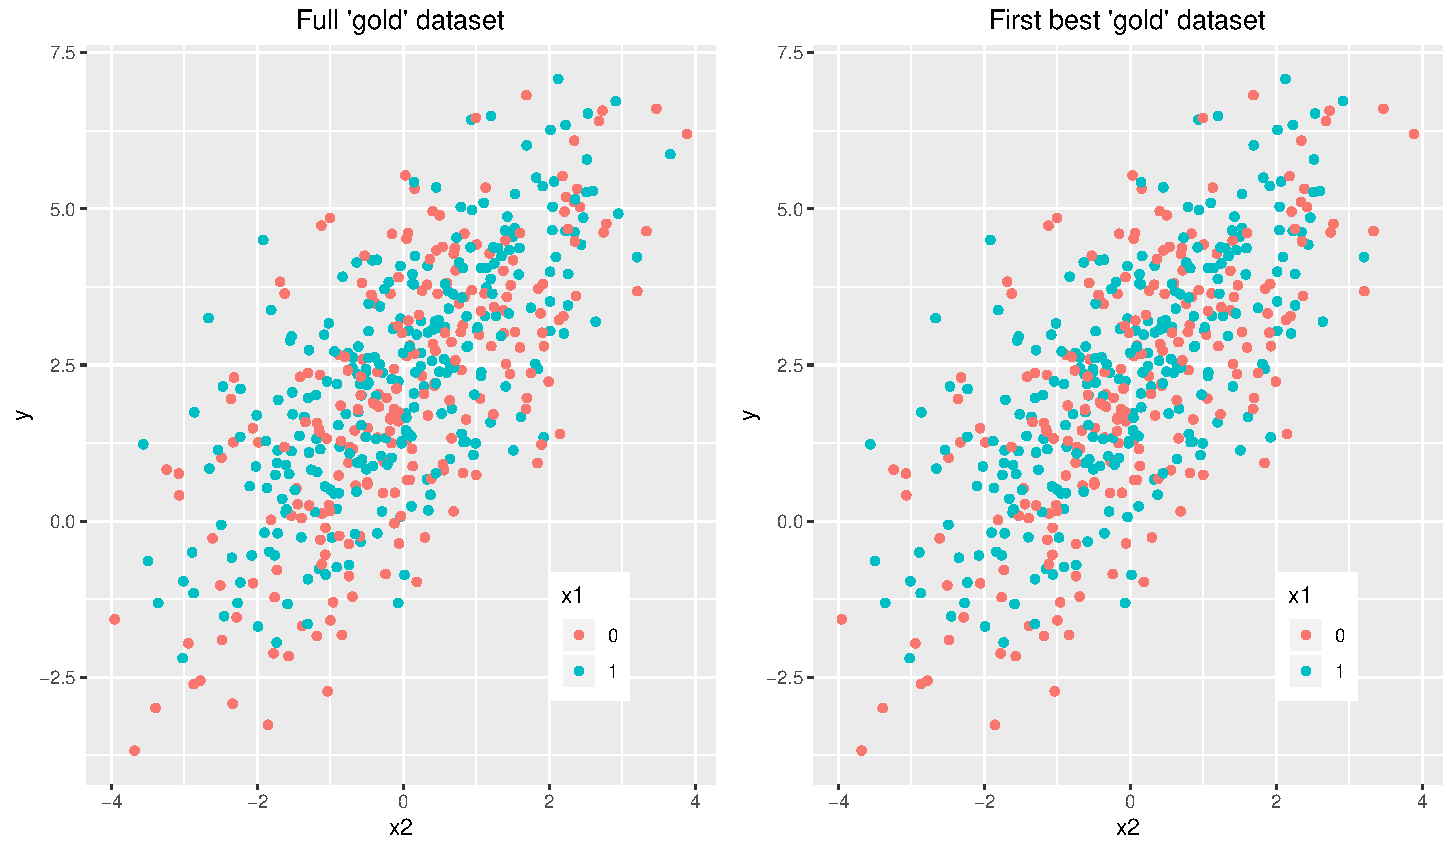
\includegraphics[height = 300pt, width=\textwidth]{./Figures/gold_data_compare.pdf}
\label{default}
\end{center}
\end{figure}

 % Massive latex Figure of synthetic dataset -- put in new file ideally
\begin{figure}
\caption{Creation of Synthetic Datasets}
\vspace{5pt}
 \begin{adjustwidth}{-.5in}{-.5in}  
\begin{tikzpicture}
\node (a) at (0,0){
\begin{tabular}{ccccccc}
\toprule
ID &  $y$ & $x_1$ & $x_2$ & First Name & Last Name & Birthday \\
\midrule
1 & $y_1$ & $x_{1,1}$ & $x_{2,1}$ & Tyler & Ashenfelter & 1915-05-13 \\
2 & $y_2$ & $x_{1,2}$ & $x_{2,2}$ & Brandon & Christensen & 1904-06-27 \\
\mc{7}{c}\vdots \\
195 & $y_{195} &$x_{1,195} & $x_{2,195}$ & Samantha & Andersen & 1914-08-18 \\
196 & $y_{196}$ & $x_{1,196}& $x_{2,196}$ & Victoria & Andersen & 1918-11-25\\
\mc{7}{c}\vdots \\ 
1000 & $y_{500}$ & $x_{1,500}$ & $x_{2,500}$ & Vicky & Anderson & 1915-04-14\\
\bottomrule
\end{tabular}};
\\
\vspace{20pt}
\\
\footnotesize{
\node[yshift=-3cm] (b) at (a.south){
\begin{tabular}{ cc }   % top level tables, with 2 rows
$x$-Datafile & $y$-Datafile \\  
% bottom left of the top level table: table 1 
\begin{tabular}{ cccc } 
\toprule
ID & $x$ & Name & Birthday \\
\midrule
2 & ($x_{1,2}, x_{2,2})$ & Branden Christenson & 1905-06-27 \\
\mc{4}{c}\dots \\
195 & ($x_{1,195},x_{2,195}$)& Samantha Anderson & 1914-08-21 \\
198 & ($x_{1,198}, x_{2,198}$)& Jon Smyth & 1918-12-20\\
\mc{4}{c}\dots \\ 
1000 & ($x_{1,1000},x_{2,1000}$) & Vic Andersn & 1915-04-14\\
\bottomrule
\end{tabular} &  % starting bottom right of the top level table
% table 2
\begin{tabular}{ cccc } 
\toprule
ID & $y$ & Name & Birthday \\
\midrule
1 & $y_1$ & Tyler Ashenfelter & 1915-05-13 \\
2 & $y_2$ & Brandon Christensen & 1904-06-27 \\
\mc{4}{c}\dots \\
195 & $y_{1,195}$ & Samantha Anderson & 1914-08-18 \\
\mc{4}{c}\dots \\ 
1000 & $y_{1000}$ & Vicky Anderson & 1915-04-14\\
\bottomrule
\end{tabular} \\
\end{tabular}};
\draw[->, thick](a)--(b);
\end{tikzpicture}
\end{adjustwidth}
\label{sample_dta}
\end{figure}%

Next, I split the ``ground truth" dataset into the $x$- and $y$-datafiles, which contain $(x_1,x_2, w_x)$ and $(y, w_y)$ values respectively.  The $y$-datafile is identical to the ground truth data, except that it excludes the variables $x_1$ and $x_2$.   The $x$-datafile contains values for 400 observations, selected at random from the full dataset. To construct $w_x$, I modify the corresponding $w_y$ by deleting characters (e.g., ``Anderson"  becomes ``Andersn"), exchanging vowels (e.g., ``Rachel" becomes ``Rachal"), or swapping English phonetic equivalents (e.g. ``Ellie" becomes ``Elie").  I also add normally distributed errors to the birth day, month, and year.  The probability of introducing an error to any one element of $w_x$ is set to mimic real-world data \footnote{add a footnote here}.  Figure \ref{sample_dta} illustrates how the $x$- and $y$-datafiles are split visually. 

%Research on record linkage appears in many fields, such as statistics, computer science, operations research, and epidemiology, under many names, such as data linkage, entity resolution, instance identication, de-duplication, merge/purge processing, and reconciliation.  As such, there are several books devoted to its study \citep{harron_book, christen2012, herzog07}, and dozens of commercial and open source systems software developed for its implementation \citep{kopcke2010}.  Although insights from other fields have been slow to reach economics, recent working papers examine the impact of different record linkage techniques on inference using historic U.S. census data \citep{abe2019, bailey2017}; and the most recent version of the Handbook of Econometrics includes a chapter on the ``Econometrics of Data Combination" \citep{RidderMoffitt}.\footnote{Similar survey papers also exist in fields outside of economics, such as epidemiology and computer science \citep{harron2018, winkler99}.  In fact, that record linkage is studied by many fields makes writing (and reading!) such surveys difficult, because authors are constantly writing the same things For example, \cite{Goldstein2012} prove similar results to those published in \cite{hirukawa2018}.}

%Record linkage techniques are broadly categorized as deterministic or probabilistic\footnote{define them here}; however, every deterministic linkage method has an equivalent probabilistic version \citep{harron2018}.  Furthermore, the first three steps of the record linkage task described above are identical for all procedures.  I begin by discussing these steps, then introduce the PRL framework, and show how it can be used to express deterministic linking rules. 


\section{Record Linkage Methods}



As observed by \cite{bailey2017}, record linkage procedures differ by the set of assumptions that motivate their use.  However, all of the procedures discussed in this paper will be studied under the following, common set of assumptions (with some departures later on):
\begin{enumerate}
\item (De-duplication) Within a given dataset, each observation refers to a distinct entity.  That is, if two observations share the same identifier, they represent two different individuals.
\item (No unobserved sample selection) The observed $x_i$ and $y_j$ are random samples conditional on $w_i$ and $w_j$, respectively.  This means that all individuals with the same identifying information have equal probability of appearing in the sample. 
\item There exists a unique $\beta_0$ that satisfies the relationship in (\ref{model}), that can be consistently estimated using standard econometric techniques if $\varphi_0$ is known.
\end{enumerate}

In total, I implement two record linkage techniques, each of which I implement while allowing multiple or enforcing single matches.  Here I provide an overview of those techniques. 
\subsection{Deterministic}
The deterministic matching algorithm described herein is based upon \cite{abe2012}.  It consists of the following steps
\begin{enumerate}
\item Clean names in $x$ and $y$ datafiles to remove any non-alphabetic characters and account for common mis-spellings and nicknames (e.g., so that Ben and Benjamin would be considered the same name).  This step usually involves the use of phonetic algorithms, such as NYSIIS or SOUNDEX.   
\item Restrict the sample to people in the $x$ datafile with unique first name, last name, and birth date combinations  
\item For each record in the $x$-datafile, look for records in the $y$-datafile that match on first name, last name, place of birth, and exact birth year.  At this point there are three possibilities 
\begin{enumerate}
\item If there is a \textit{unique} match, this pair of observations is considered a match.
\item If there are multiple potential matches in the $y$-datafile with the same year of birth, the observation is discarded. 
\item If there are no matches by exact year of birth, the algorithm searches for matches within $\pm$ 1 year of reported birth year, and if this is unsuccessful, it looks for matches within $\pm$ 2 years.  In each of these steps, only unique matches are accepted.  If none of these attempts produces a unique match, the observation is discarded.
\end{enumerate}
\item Step 3 is repeated for each record in the $y$-datafile, after which the intersection of the two matched samples is taken. 
\end{enumerate}

An interesting quirk of this algorithm is that one person could have a unique exact year match, but then multiple matches with birth years off by 1; this person is included when a unique match is desired.  But if the unique match with zero year difference were not present, then the observation would be dropped. 

\subsection{Probabilistic Record Linkage}
The probabilistic record linkage technique implemented in this paper are based on seminal work by \cite{fellegi69}, which views record linkage as a classification problem.  As before, let $\{x_i, w_i\}$, $i=1,\dots,N_x$ denote the observations in a dataset $X$; and $\{y_j,w_j\}$, $j=1, \dots N_y$, denote the observations in a dataset $Y$.  The space of record pairs $X \times Y$ can be divided into two disjoint sets, \textit{matches} $(M)$ and \textit{non-matches} $(U)$, defined as
\begin{align*} M &= \{ (i,j) \in X\times Y: j \in \varphi(i) \} \\ U &= \{(i,j) \in X\times Y:  j \notin\varphi(i)\}\end{align*} 

 To determine whether a record pair belongs to $M$ or $U$, the pair is evaluated according to $K$ different comparison criteria, which result from comparing $w_i$ and $w_j$.  These comparisons are represented in a \textit{comparison vector}, $$\mathbf{\gamma_{ij}}= (\gamma_{ij}^1, \dots, \gamma_{ij}^{k}, \dots, \gamma_{ij}^K)$$  where each comparison field $\gamma_{ij}^{k}$ may be binary-valued, as in ``$i$ and $j$ have the same birthday" and ``$i$ and $j$ have the same last name," or use ordinal values to indicate partial agreement between strings.

The probability of observing a particular configuration of $\gamij$ can be modeled as arising from the mixture distribution:
\begin{equation}
P(\gamij) = P(\gamij | M) p_M + P(\gamij | U) p_U 
\label{mm}
\end{equation}
where $P(\gamij | M)$ and $P(\gamij | U)$ are the probabilities of observing the pattern $\gamij$ conditional on the record pair $(i,j)$ belonging to $M$ or $U$, respectively.  The proportions $p_M$ and $p_U = 1-p_M$ are the marginal probabilities of observing a matched or unmatched pair.  Applying Bayes' Rule, we obtain the probability of $(i,j) \in M$ conditional on observing $\gamij$,
\begin{equation} P(M | \gamij) = \frac{p_M P(\gamij | M)}{P(\gamij)} \label{bayes} \end{equation}
Thus, if we can estimate $p_M$, $P(\gamij | M)$ and $P(\gamij | U)$, then we can estimate the probability that any two records refer to the same entity using (\ref{bayes}).   These probabilities can then be used to designate pairs as matches, or to estimate the false positive rate associated with a particular match configuration using the formulas in \cite{fellegi69}.  

Note that when $X$ or $Y$ is large, constructing comparison vectors for all $N_x\times N_y$ possible pairs can be computationally intensive.   In practice, researchers solve this problem by partitioning $X\times Y$ into ``blocks," such that comparison vectors are only constructed for records within the same block, and records in different blocks are assumed to be non-matches. Importantly, the blocking variables should be recorded with minimal error, otherwise blocking may adversely affect the Type II error rate. 

\textbf{Example 1 (cont'd).} This paper assumes that no blocking is used; or, alternatively, that records are already divided into blocks that can be analyzed independently using the methods outlined below.  

Another difficulty arises from the fact that there are at least $2^K -1$ possible configurations of $\gamij$.  While in principle we could model $P(\gamij | M)$ and $P(\gamij | U)$ as
\begin{align*} (\gamma_{ij}^1, \dots, \gamma_{ij}^K) \  |\  M &\sim \text{Dirichlet}(\mathbf{\delta_M})\\
 (\gamma_{ij}^1, \dots, \gamma_{ij}^K) \  |\  U &\sim \text{Dirichlet}(\mathbf{\delta_U}) \end{align*}
but the parameters $\mathbf{\delta_M}$ and $\mathbf{\delta_U}$ may be high-dimensional.  However, if the comparison fields $\gamma_{ij}^{k}$ are independent across $k$ conditional on match status, then the number of parameters used to describe each mixture class can be reduced to $K$ by factoring:
 \begin{equation} 
 P(\gamma_{ij} | C) = \prod_{k=1}^K P(\gamma_{ij}^{k} | C)^{\gamma_{ij}^{k}}(1-Pr(\gamma_{ij}^{k} | C))^{1-\gamma_{ij}^{k}} \hspace{20pt} C\in \{M, U\} 
 \label{eq:condInd}
 \end{equation}
 Alternatively, dependence between fields can be modeled using log-linear models; however, I assume conditional independence to ease computation.  

\textbf{Example 1 (cont'd)}.  Errors are constructed to satisfy this assumption

\section{Estimation Methods}
This section provides an overview of the estimation methods I compare for analyzing the matched datasets. 
\subsection{OLS Bias Correction}
 \cite{sw1993} and \cite{lahiri05} propose techniques for correcting the bias from mismatched pairs in linear regression.  They assume that the matching procedure produces $n$ pairs $(x_i, z_i)$, where $z_i$ may or may not correspond to $y_i$, yet the true $y_i$ is included among the matches.   Hence, 
$$z_i = \begin{cases} y_i & \text{with probability $q_{ii}$} \\ y_j & \text{with probability $q_{ij}$ for $j\neq i,\ j = 1,\dots,n $} \end{cases}$$ 
and $\sum_{j=1}^n q_{ij} = 1, \ i=1,\dots, n$.  Estimating (\ref{model}) using $z_i$ as the dependent variable yields the naive least squares estimator, 
\begin{equation} \hat{\beta}_N = (X'X)^{-1} X'z \label{naive} \end{equation}
which is biased.   Denoting $q_i = (q_{i1}, \dots, q_{in})'$ and $Q = (q_1, \dots, q_n)'$, we can write the bias of $\hat{\beta}_N $ as
$$\text{bias}(\hat{\beta}_N) = [(X'X)^{-1} X'QX - I] \beta $$ 
 since $E[z_i] = E[q_i'y]  = q_i'X\beta =  \sum_{j=1}^{n} q_{ij} x_j'\beta $.  

To reduce the bias of $\hat{\beta}_N$, \cite{sw1993} observed that 
\begin{equation} \text{bias} (\hat{\beta}_N | y) = E[(\hat{\beta}_N - \beta) | y ] = (X'X)^{-1} X'B \label{bias} \end{equation}
where $B = (B_1, \dots, B_n)'$ and $B_i = (q_{ii}-1)y_i + \sum_{j\neq i } q_{ij} y_j = q_i'y - y_i$, which is the difference between a weighted average of responses from all observations and the actual response $y_i$.  The authors suggest estimating (\ref{bias}) using the first and second highest elements of the vector $q_i$, so that $\hat{B}_i^{TR} = (q_{ij_1} - 1) z_{j_1} + q_{ij_2} z_{j_2}$, and 
\begin{equation} \hat{\beta}_{SW} = \hat{\beta}_N - (X'X)^{-1} X' \hat{B}^{TR} \label{sw}\end{equation}
The estimator can incorporate any number of elements of $q_i$, but, if the probability is high that the best candidate link is the true link, then the truncation  results in a very small bias. 

Alternatively,  \cite{lahiri05} use the fact that $E(z_i) = w_i'\beta$, where $w_i = q_i'X_i\beta$, to construct the unbiased estimator:
$$ \hat{\beta}_U = (W'W)^{-1} W'z$$ 
where $W = (w_1, \dots, w_N)'$.  To construct $\hat{\beta}_U$ in practice, they also recommend using a truncated version of $W$, with $w_i^{TR} = q_{ij_1} x_{j_1} + q_{ij_2} x_{j_2}$.

For both methods, the values $q_{ij}$ are typically calculated using (\ref{bayes}) and parameter values $\psi = \{p_M, P(\gamij | M)$, and $P(\gamij |U)\}$. Thus, we can write the estimators $\hat{\beta}_{SW} = \hat{\beta}_{SW}(\psi)$ and $\hat{\beta}_U = \hat{\beta_U}(\psi)$.  In practice, $\psi$ is unknown, and a reasonable estimator $\hat{\psi}$ must be used.   Details on how to estimate $\hat{\psi}$ are provided in the next section.   Importantly, $\hat{\beta}_U(\hat{\psi})$ is unbiased whenever $\hat{\psi}$ is independent of $z$, which occurs if errors in the matching variables (which determine the distribution of $\hat{\psi}$ are independent of the response variable $y$.  Unfortunately, this assumption is unlikely to hold in many economic applications, such as \cite{nq2015}, where $y$ indicates whether a person's recorded ethnicity changes between survey years, but data quality significantly differs for individuals with different values of $y$.  

\subsection{Multiple match WLS}

 \cite{ahl2019} propose a GMM estimator that uses data where each observation $x_i$ is linked to $L_i$ equally likely, potential outcomes, denoted $\{y_{i\ell}\}_{\ell=1}^{L_i}$.  Importantly, their methods require that (i) the true outcome is included among the set of possible matches, (ii) each of the possible matches is equally likely to be the true match, and (iii) that the observations $x_i$ and $\{y_{i\ell}\}_{\ell=1}^{L_i}$ are random samples from their marginal distributions conditional on $(w_i, L_i)$.  
 
Under these assumptions, the authors show how to construct an unbiased and consistent estimator $\hat{\beta}$ by considering the smoothed regression:
\begin{equation} 
\sum_{\ell=1}^{L_i} y_{i\ell} - (L_i - 1)g(w_i, L_i) = x_i'\beta + u_i  \end{equation}

\noindent where $g(w_i, L_i) = E[y_{i\ell} | w_i, L_i ]$, $u_i = \varepsilon_i + \sum_{\ell=1}^{L_i}\nu_{i\ell}$, and $\nu_{i\ell} = y_{i\ell} - E[y_{i\ell} | w_i, L_i ]$. 

If, additionally, $E[\varepsilon_i^2 | w_i, L_i] = \sigma_{\varepsilon}^2$ and $E[\nu_{i\ell} | z_i, L_i] = \sigma_{\nu}^2$ then $\hat{\beta}$ can be estimated efficiently using weighted least squares, with $\sigma(X_i) = \sigma_{\varepsilon}^2 + (L_i - 1)\sigma_{\nu}^2$, and
\begin{equation}
\hat{\beta}^{WLS} = \left(\sum_{i=1}^N \frac{x_ix_i'}{\sigma(X_i)}\right)^{-1}\left(\sum_{i=1}^N \frac{x_i}{\sigma(X_i)}\left(\sum_{\ell=1}^{L_i} y_{i\ell} - (L_i - 1) g(w_i, L_i)\right)\right)
\end{equation}
which can be estimated in two-steps, where the first step involves estimating $\hat{g}(\cdot)$ and $\hat{\sigma}(X_i)$.  The resulting estimator is consistent and asymptotically normal under the regularity conditions described in \cite{ahl2019}. 

Assumption (iii) rules out the possibility of unobserved sample selection, in the sense that all individuals with the same identifying information have equal probability of appearing in the sample.  This assumption would be violated if, for example, higher income individuals have a greater probability of appearing in the sample (unless $w_i$ includes income).   However, unlike the OLS bias correction estimators, the methods here explicitly correct for any dependence between the outcome variable and the matching variables $w_i$ and the parameters of the matching procedure, insofar as they are captured by $L_i$.  

[This suggests that the AHL (2019) estimator may be more robust when $L_i$ is correlated with $x_i$..]

\section{Implementation}

\subsection{Matching Algorithms}
\subsubsection*{Implementation Notes}
When applying the algorithm with the synthetic data, I make the following alterations:
\begin{enumerate}
\item I standardize the names by using the nysiis function in R.  I do not need to correct for nicknames, because of how I have generated the names. 
\item  I restrict the all observations with unique first name, last name, date of birth, and $(x_1, x_2)$ combinations.  
\item I only perform two-way matches -- that is I repeat the process for all observations in the $y$ datafile and take the intersection of the matches).  Does this change my results (check)?
\item  When allowing for multiple matches, I count as matches all record pairs with the same name, and the difference in recorded birth years is within two (or five) years.  That is, I designate all potential matches that arise in Step 3 as matches. 
\end{itemize}


\textbf{Example 1 (cont'd).} Here are the differences that arise with two-way vs. not, nysiis vs. not, etc. 


\subsubsection*{PRL}  Since membership to $M$ or $U$ is not actually observed, a convenient way of simultaneously estimating $p_M, p_U$ and classifying record pairs as matches or non-matches is via mixture modeling, with mixture distributions $P(\gamij | M)$ and $P(\gamij | U)$.   %This approach was suggested by Bayesian approaches to record linkage have been suggested by Larsen (1999a, 2002, 2004, 2005), Fortini et al. (2002, 2000), and McGlinchy (2004).

For convenience, denote $p_{M\ell} = P(\gamma_{ij}^{\ell} | M)$ and $ p_{U\ell} = P(\gamma_{ij}^{\ell} | U)$.  Assuming conditional independence across $\ell$ (and global parameters that do not vary by block, if using blocked records), a convenient prior distribution is the product of independent Beta distributions,
 \begin{gather*}
 p_M \sim \text{Beta}(\alpha_M, \beta_M) \\
 p_{M\ell} \sim \text{Beta}(\alpha_{M\ell}, \beta_{M\ell}), \ \ell = 1,\dots, L \\
  p_{U\ell} \sim \text{Beta}(\alpha_{U\ell}, \beta_{U\ell}), \ \ell = 1,\dots, L 
 \end{gather*}
 For $i=1,\dots,n_1 \in X_1$, $j = 1, \dots, n_2 \in X_2$ define the parameter of interest as,
$$I_{ij} = \begin{cases} 1, & \text{if records $i\in X_1$ and $j\in X_2$ refer to the same entity;} \\ 0, & \text{otherwise} \end{cases} $$  
If $\params$ are known, then $P(I_{ij} = 1 | \gamij \params)$ is distributed as in (\ref{bayes}).  Alternately, if the match indicators $\mathbf{I}$ were known, the posterior distributions of $\left(p_M, \mathbf{p_{M\ell}, p_{U\ell}}\right)$ would be:

% pM | I
\begin{equation}
p_M | I \sim \text{Beta}\left(\alpha_M + \sum_{(i,j)} I_{ij},\ \beta_M + \sum_{(i,j)} (1- I_{ij})\right) 
\label{eq:pM}
\end{equation}

% pML | I 
\begin{equation}
p_{M\ell} | I \sim \text{Beta}\left(\alpha_{M\ell} + \sum_{(i,j)} I_{ij}\gamma_{ij}^{\ell},\ \beta_{M\ell} + \sum_{(i,j)} I_{ij} (1-\gamma_{ij}^{\ell})\right), \hspace{10pt} \ell = 1,\dots, L
\label{eq:pML}
\end{equation}

%pUL | I 
\begin{equation}
p_{U\ell} | I \sim \text{Beta}\left(\alpha_{U\ell} + \sum_{(i,j)}(1-I_{ij})\gamma_{ij}^{\ell},\ \beta_{U\ell} + \sum_{(i,j)}(1-I_{ij})(1-\gamma_{ij}^{\ell})\right), \hspace{10pt} \ell = 1,\dots, L
\label{eq:pUL}
\end{equation}

% \[ P(\mathbf{\Gamma} | \mathbf{I}) &= \prod_{(i,j)} P(\gamij | M)^{I_{ij}} P(\gamij | U)^{1-I_{ij}} \]

Based on these ideas, \cite{larsen_rubin_2001} proposed a Bayesian version of record linkage for the mixture model approach, that uses a Gibbs Sampling scheme\footnote{See Appendix \ref{app:simple_gibbs}} for simulating the posterior distribution of $I,\params$. 



\subsection{Estimation Algorithms}  

For LL, $z$ requires single matches.  So I pick at random one of the highest posterior matches and call that $z$. 

Standard errors for $\hat{\beta}_{SW}$ are calculated using the formula. 
Standard errors for $\hat{\beta}_{LL}$ are calculated via the parametric bootstrap described in \cite{lahiri05}.  


For AHL (2019), I use nearest neighbors applied to the datasets $\{x_i, \{y_{i\ell}\}_\ell, w_i \}$ that are outputted by the matching algorithms above.  That means, I implement the method as if the researcher only observes the matched dataset.  

\section{Results}
I test three DGPs. The first was described above.  The second allows for correlation  between $x_1$ and the probability of an error.  The third will allow for correlation between $y$ and the probability of an error. 

The $y$ are generated according to the same DGP described above; that is the true $\beta_0 = (2, 0.5, 1)$.  I compare my results to an oracle linkage method (``first best"), which would successfully link all 400 $x$ observations to their correct $y$.  This produces $\hat{\beta}_{FB}$, which is shown in the table below:
% results here

%% Matching Algorithm Comparison
% Match Rate Table 
\begin{table}[h!]
\let\center\empty
\let\endcenter\relax
\centering
\caption{Match rate for matching algorithms}
\vspace{10pt}
\resizebox{0.6\textwidth}{!}{
\begin{tabular}{cccccc}
\toprule
Method & Match Rate & \# Matches & Type I & Type II & P(Contains True)\\
\midrule
ABE (Single) & 0.71 (0.02) & 356.50 (10.60) & 0.03 (0.01) & 0.26 (0.02) & 0.97 (0.01)\\
ABE (Multi) & 0.79 (0.02) & 505.08 (17.30) & 0.23 (0.02) & 0.20 (0.02) & 0.99 (0.01)\\
PRL (Single) & 0.74 (0.02) & 369.15 (9.65) & 0.11 (0.02) & 0.15 (0.03) & 0.89 (0.02)\\
PRL (Multi) & 0.74 (0.02) & 435.65 (14.94) & 0.18 (0.02) & 0.23 (0.02) & 0.97 (0.01)\\
\bottomrule
\end{tabular}
}
\end{table}

% Distribution of  L_i
\begin{figure}[h!]
\begin{center}
\caption{Distribution of number of matches produced by multi-matching algorithms}
\vspace{-20pt}
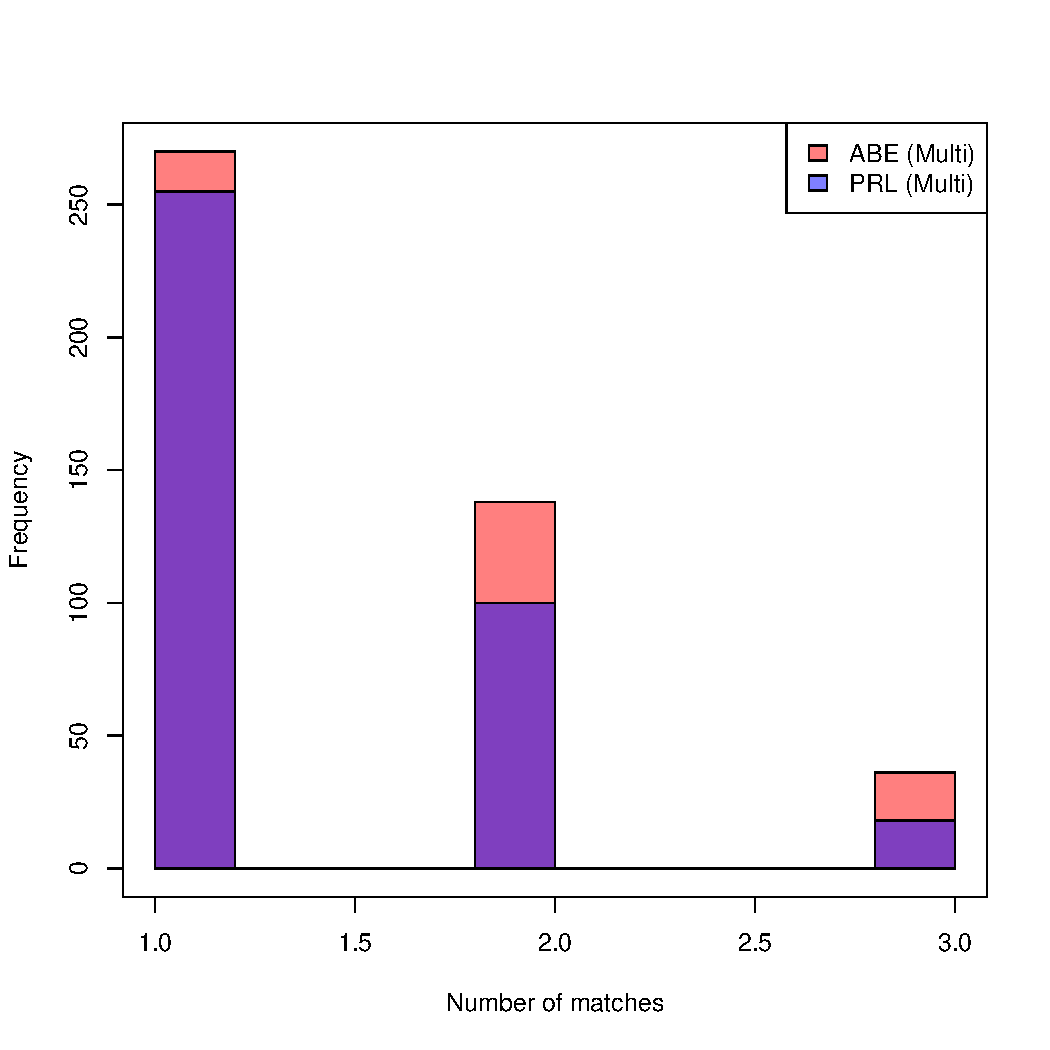
\includegraphics[width=0.7\textwidth]{./Figures/match_hist.pdf}
\caption{default}
\label{default}
\end{center}
\end{figure}

% Naive OLS Table
\begin{table}[h!]
\let\center\empty
\let\endcenter\relax
\centering
\caption{Naive OLS for all of the matchings}
\resizebox{\textwidth}{!}{
% Table created by stargazer v.5.2.2 by Marek Hlavac, Harvard University. E-mail: hlavac at fas.harvard.edu
% Date and time: Wed, Oct 02, 2019 - 11:22:55
\begin{tabular}{@{\extracolsep{5pt}}lccccc} 
\\[-1.8ex]\hline 
\hline \\[-1.8ex] 
 & \multicolumn{5}{c}{\textit{Dependent variable:}} \\ 
\cline{2-6} 
\\[-1.8ex] & \multicolumn{5}{c}{y} \\ 
 & First Best & ABE (Single) & ABE (Multi) & PRL (Single) & PRL (Multi) \\ 
\hline \\[-1.8ex] 
 x1 & 0.408$^{***}$ & 0.413$^{**}$ & 0.369$^{**}$ & 0.587$^{***}$ & 0.357$^{**}$ \\ 
  & (0.143) & (0.172) & (0.153) & (0.180) & (0.168) \\ 
  & & & & & \\ 
 x2 & 1.096$^{***}$ & 1.010$^{***}$ & 0.905$^{***}$ & 0.975$^{***}$ & 0.930$^{***}$ \\ 
  & (0.052) & (0.062) & (0.056) & (0.065) & (0.062) \\ 
  & & & & & \\ 
 Constant & 2.079$^{***}$ & 2.106$^{***}$ & 2.100$^{***}$ & 1.932$^{***}$ & 2.091$^{***}$ \\ 
  & (0.102) & (0.125) & (0.109) & (0.131) & (0.122) \\ 
  & & & & & \\ 
\hline \\[-1.8ex] 
Observations & 400 & 327 & 454 & 311 & 373 \\ 
R$^{2}$ & 0.534 & 0.455 & 0.367 & 0.429 & 0.384 \\ 
Adjusted R$^{2}$ & 0.532 & 0.452 & 0.364 & 0.425 & 0.381 \\ 
\hline 
\hline \\[-1.8ex] 
\textit{Note:}  & \multicolumn{5}{r}{$^{*}$p$<$0.1; $^{**}$p$<$0.05; $^{***}$p$<$0.01} \\ 
\end{tabular} 
}
\end{table}

\subsection{Matching step}
\begin{figure}[htbp]
\caption{Matches}
\begin{center}


\label{default}
\end{center}
\end{figure}

% latex table generated in R 3.5.1 by xtable 1.8-3 package
% Mon Sep 30 16:31:01 2019
\begin{table}[ht]
\centering
\caption{}
\vspace{5pt}
\begin{tabular}{rlrrr}
  \hline
 & method & nMatches & pCorrect & nUniqueX \\ 
  \hline
1 & abe\_single & 338 & 0.96 & 338 \\ 
  2 & abe\_multi & 479 & 0.77 & 375 \\ 
  3 & prl\_single & 335 & 0.87 & 335 \\ 
  4 & prl\_multi & 397 & 0.79 & 335 \\ 
   \hline
\end{tabular}
\end{table}

\subsection{Estimation Results}
\begin{table}[htdp]
\caption{Parameter estimates for different matched datasets and estimation procedures}
\begin{center}
\begin{tabular}{|c|c|}

\end{tabular}
\end{center}
\label{default}
\end{table}%


\section{Conclusion}
Borrow from the Bayesian Record Linkage. 


Merging datasets with imperfect identifiers occurs frequently in projects that use historical U.S. data sources prior to the introduction of Social Security Numbers.  For example, \cite{aizer2016} link children listed on Mothers' Pension program welfare applications from 1911-1935 with Social Security Death Master File records from 1965-2012 using individuals' names and dates of birth.  Although the authors match 48 percent of children to a unique death record, and 4 percent to multiple possible records, 48 percent of observations remain unmatched\footnote{The authors estimate that at least 32 percent of individuals in the Mothers' Pension program data died before 1965, and therefore should have no match in the 1965-2012 data.}.  To avoid dropping the 52 percent of observations with zero or multiple matches, \cite{aizer2016} estimate hazard models using methods from \cite{ahl2019} that allow observations to be associated with multiple, equally likely, outcomes.  

The methods used by \cite{aizer2016} illustrate how inference using linked data requires joint assumptions for the matching and estimation steps.  Under different assumptions, the authors could have generated a ``composite match" equal to the average of the linked observations \citep{bleakley2016}, or constructed bounds on the parameter of interest using different configurations of matched data \citep{nq2015}.   This example also shows how the outputs of the matching process determine which estimation tools are available.  Had the authors used probabilistic record linkage methods to link the data, they could have used the robust OLS estimators from \cite{lahiri05}, or prior-informed imputation for missing records proposed by \cite{Goldstein2012}.   


\newpage
\singlespacing
\bibliography{./Deadlines/proposal_bib} 
\bibliographystyle{aer}

\end{document}